\documentclass{article}
\usepackage[left=1in, right=1in, top=1in, bottom=1in]{geometry}
\usepackage{mathexam}
\usepackage{amsmath}
\usepackage{graphicx,subcaption}
\usepackage{booktabs}
\usepackage{enumitem}
\usepackage{atbegshi}% http://ctan.org/pkg/atbegshi
\usepackage[ruled,linesnumbered]{algorithm2e}
\AtBeginDocument{\AtBeginShipoutNext{\AtBeginShipoutDiscard}}

%\ExamClass{Sample Class}
%\ExamName{Sample Exam}
%\ExamHead{\today}

%\let\ds\displaystyle

\begin{document}

\begin{titlepage}
	\vspace*{\stretch{1.0}}
	\begin{center}
		\Large\textbf{Rectifying Bound}\\
		\large\textit{20 August 2018}
	\end{center}
	\vspace*{\stretch{2.0}}
\end{titlepage}












\begin{algorithm}
	\SetAlgoVlined
	\DontPrintSemicolon
	%This is to hide Begin keyword
	\SetKwBlock{Begin}{}{end}
	\KwIn{Set of views V and result set $S$ize k }
	\KwOut{Result set $ S \leq V $, size S = k}  
	\SetKwFunction{FgetL}{getL}
	\SetKwFunction{FgetMaxPI}{getMaxPI}
	$S \leftarrow $ two most distant views\;
	$X \leftarrow  \left[V \backslash S\right]$\;
	
	
	
	\SetKwFunction{FgetL}{getL}
	\SetKwProg{Fn}{function}{:}{}
	\Fn{\FgetL{$f$,$S$, $X$,$L$}}{
		\For{$X_i$ in set $X$}{
			\For{$S_j$ in set $S$}{
				$ d  \leftarrow setDist\left(X_i,S \right) $\;
				%$ 	X' \leftarrow [ X_i, d]$\;
				$ 	L.append([ X_i, d])$\;
			}
		}
		$ 	L \leftarrow sorted\_by\_d(L) $\;
		
		\KwRet L\;
	}

%\SetKwFunction{FgetMaxPI}{getMaxPI}
%\SetKwProg{Fn}{function}{:}{}
%\Fn{\FgetMaxPI{$f$,$S$, $X$,$max_b$}}{
%	$samples \leftarrow get\_samples\_PI(X)$\;
%	$maxI\_S \leftarrow get\_maxI(S)$\;
%	$maxI\_samples \leftarrow get\_maxI(samples)$\;
%	
%	\If{ $ maxI\_S > maxI $}{
%		$ maxI \leftarrow maxI\_S$
%	}
%	\If{ $ maxI\_samples> maxI $}{
%		$ maxI \leftarrow maxI\_samples$
%	}
%	$max_b \leftarrow maxI$		
%	
%	\KwRet\;
%}
	
	%$ rectify \leftarrow False $\;
	$ L_{base}, S_{base},S'_{base}   \leftarrow getL(S,X), S, S \cup L[X_1] $\;
	$max_b \leftarrow getMaxPI(S,X) $	\;
	$rectify, step\_back \leftarrow False, 3 $	\;
	\;
	\While{$i < k$}{

		
	%	$ S' \leftarrow S $\;
		\If{$rectify = False$}{
		$ L \leftarrow getL(S,X) $\;
	$ S' \leftarrow S \cup L[X_1] $\;	
	}
		\For{$L_i$ in $L$}{
			\If{$rectify=True$}{
			 $start\; loop\; at\; L[min_d]$}
			\If{ $ F\left(S'\right) < F\left(S \cup X_i, max_b\right) $}{
					$ I \leftarrow get\_I\_score(X_i) $\;
			\If{ $ F\left(S'\right) < F\left(S \cup X_i, I\right) $}{
			$ S'  \leftarrow S \cup X_i $  \;
		}
		\eIf{ $ I > max_b $}{
			$ max_b \leftarrow I $\;
			$ rectify = True $\;
			$ break (Out\ of\ Loop) $\;
		}{
			$ rectify = False $\;
			
		}
			}
		
		
			
		}
	
		%$ S  \leftarrow S'$\;
	
		
		\eIf{ $ rectify == True $}{
		\eIf{$step\_back < i - 2$}{
%		$ S, S' \leftarrow S_{base} $ \;
%	$ L \leftarrow L_{base} $ \;
%	$i \leftarrow  2$ \;	
	$ G \leftarrow fetchTempResult(i- step\_back)$\;
$ S, S' \leftarrow G[S], G[S'] $ \;
$ L \leftarrow G[L] $ \;
$i = i- step\_back  $\;
	}{
		$ S, S' \leftarrow S_{base},S'_{base}  $ \;
	$ L \leftarrow L_{base} $ \;
	$i \leftarrow  2$ \;	

}
		
		
	}{
	$ storeTempResult(i, S, S', L, min_d)$\;
	$ S \leftarrow S' $ \;
		$i = i + 1  $\;
}
			
			
	
		

		
	
	
		
		%
		%\If{ $ F\left(S'\right) > F\left(S\right) $}{
		%	$ S  \leftarrow S'$
		%	$  improve \leftarrow  True $\;
		%	
		%	}{
		%		$improve \leftarrow  False $\;
		%	
		%	}
	}
	$return\; S$
	\caption{\textit{DiVE} Greedy Pruning Rectifying}\label{DiVE-Greedy-Pruning-Rectifying}
\end{algorithm}


% Pruning Pseudocode

\begin{algorithm}
	\SetAlgoVlined
	\DontPrintSemicolon
	%This is to hide Begin keyword
	\SetKwBlock{Begin}{}{end}
	\KwIn{Set of views V and result set $S$ize k }
	\KwOut{Result set $ S \leq V $, size S = k}  
 	\SetKwFunction{FgetL}{getL}
	$S \leftarrow $ Result set of only diversity\;
	$X \leftarrow  \left[V \backslash S\right]$\;

	
	
\SetKwFunction{FgetL}{getL}
\SetKwProg{Fn}{function}{:}{}
\Fn{\FgetL{$f$,$S$, $X$,$L$}}{
	\For{$X_i$ in set $X$}{
		\For{$S_j$ in set $S$}{
			$ d  \leftarrow setDist\left(X_i,S \right) $\;
			%$ 	X' \leftarrow [ X_i, d]$\;
			$ 	L.append([S_j, X_i, d])$\;
		}
	}
	$ 	L \leftarrow sorted\_by\_d(L) $\;
	
	\KwRet L\;
}

%\SetKwFunction{FgetMaxPI}{getMaxPI}
%\SetKwProg{Fn}{function}{:}{}
%\Fn{\FgetMaxPI{$f$,$S$, $X$,$max_b$}}{
%	$samples \leftarrow get\_samples\_PI(X)$\;
%	$maxI\_S \leftarrow get\_maxI(S)$\;
%	$maxI\_samples \leftarrow get\_maxI(samples)$\;
%	
%	\If{ $ maxI\_S > maxI $}{
%		$ maxI \leftarrow maxI\_S$
%	}
%	\If{ $ maxI\_samples> maxI $}{
%		$ maxI \leftarrow maxI\_samples$
%	}
%	$max_b \leftarrow maxI$		
%	
%	\KwRet\;
%}

$F_{current}, counter, step\_back \leftarrow 0,0, 3$\;
$ improve, rectify \leftarrow  True, False $\;
$ S_{base}, L_{base}   \leftarrow S, getL(S,X) $\;
	$max_b \leftarrow getMaxPI(S,X) $	\;
\;
	\While{$improve = True$}{
		$counter = counter + 1$ \;	
			\If{$rectify = False$}{
				$L \leftarrow getL(S,X)$ \;	
		$ S' \leftarrow S $\;

		}
	

		\For{$L_i$ in $L$}{
				\If{$rectify=True$}{
				$start\; loop\; at\; L[min_d]$}
			\If{ $ F\left(S'\right) < F\left(S \backslash S_j \cup X_i, max_b\right) $}{
			%	$ 	L'.append(L_i)$\;
			
			$ I \leftarrow get\_I\_score(X_i) $\;
			\If{ $ F\left(S'\right) < F\left(S\backslash S_j \cup X_i, I\right) $}{
				$ S'  \leftarrow S \backslash j \cup X_i $  \;
			}
			\eIf{ $ I > max_b $}{
				$ max_b \leftarrow I $\;
				$ rectify = True $\;
				$ break (Out\ of\ Loop) $\;
			}{
			$ rectify = False $\;
		}
		}
		}
		
		
		\eIf{$rectify == True$}{
			\eIf{$step\_back < counter $}{
	
					$ G \leftarrow fetchTempResult(counter - step\_back)$\;
				$ S, S' \leftarrow G[S], G[S'] $ \;
				$ L \leftarrow G[L] $ \;
			}{
					$ S, S' \leftarrow S_{base} $ \;
					$ L \leftarrow L_{base} $ \;
					$counter = 0$
	}
			$  improve \leftarrow  True $\;
			
			
		}{
		
			$ storeTempResult(counter, S, S', L, min_d)$\;

\If{ $ F\left(S'\right) > F\left(S\right) $}{
	$ S  \leftarrow S'$\;
	
}	

	\eIf{ $ F\left(S\right) > F_{current} $}{
	$ F_{current}  \leftarrow F\left(S\right) $\;
	$  improve \leftarrow  True $\;
	
}{
	$improve \leftarrow  False $\;
	
}

}
	

	
		
		%
		%\If{ $ F\left(S'\right) > F\left(S\right) $}{
		%	$ S  \leftarrow S'$
		%	$  improve \leftarrow  True $\;
		%	
		%	}{
		%		$improve \leftarrow  False $\;
		%	
		%	}
	}
	$return\; S$
	\caption{\textit{DiVE} dSwap Pruning Rectifying}\label{DiVE-dSwap-Pruning-Rectifying}
\end{algorithm}




\section{Correcting wrong maximum bound in adaptive pruning scheme}


In order to reduce costs, our DiVE schemes utilize the importance score bound to do pruning. There are two pruning techniques proposed: 1) static bound and 2) adaptive bound. In the static bound, the theoritical maximum bound ($ \sqrt{2} $) is used and this bound will not be changed until the end of running. Meanwhile, adaptive used the estimation of maximum bound as the first, then this bound is updated while there is a higher maximum bound found. 


To know when the bound should be updated, samping based on prediction interval is used. Before running the program, user needs to defined what PI that she wants to use. For instance, while users set PI to 80 means after 9 views are executed, then the current bound will be updated to the maximum importance score which have seen so far. In the algorithm \ref{DiVE-Greedy-Pruning-Rectifying} and \ref{DiVE-dSwap-Pruning-Rectifying}, $getMaxPI(S,X)$ is the function to get the estimated maximum bound from some number of executed views based on PI. Generally, PI can be defined as following: 

\begin{itemize}[noitemsep]
	\item PI80: need to execute 9 views
	\item PI85: need to execute 12 views
	\item PI90: need to executes 20 views
	\item PI95: need to executes 40 views
	\item PI97: need to executes 60 views
\end{itemize}




%
%\begin{figure}
%	\begin{center}
%		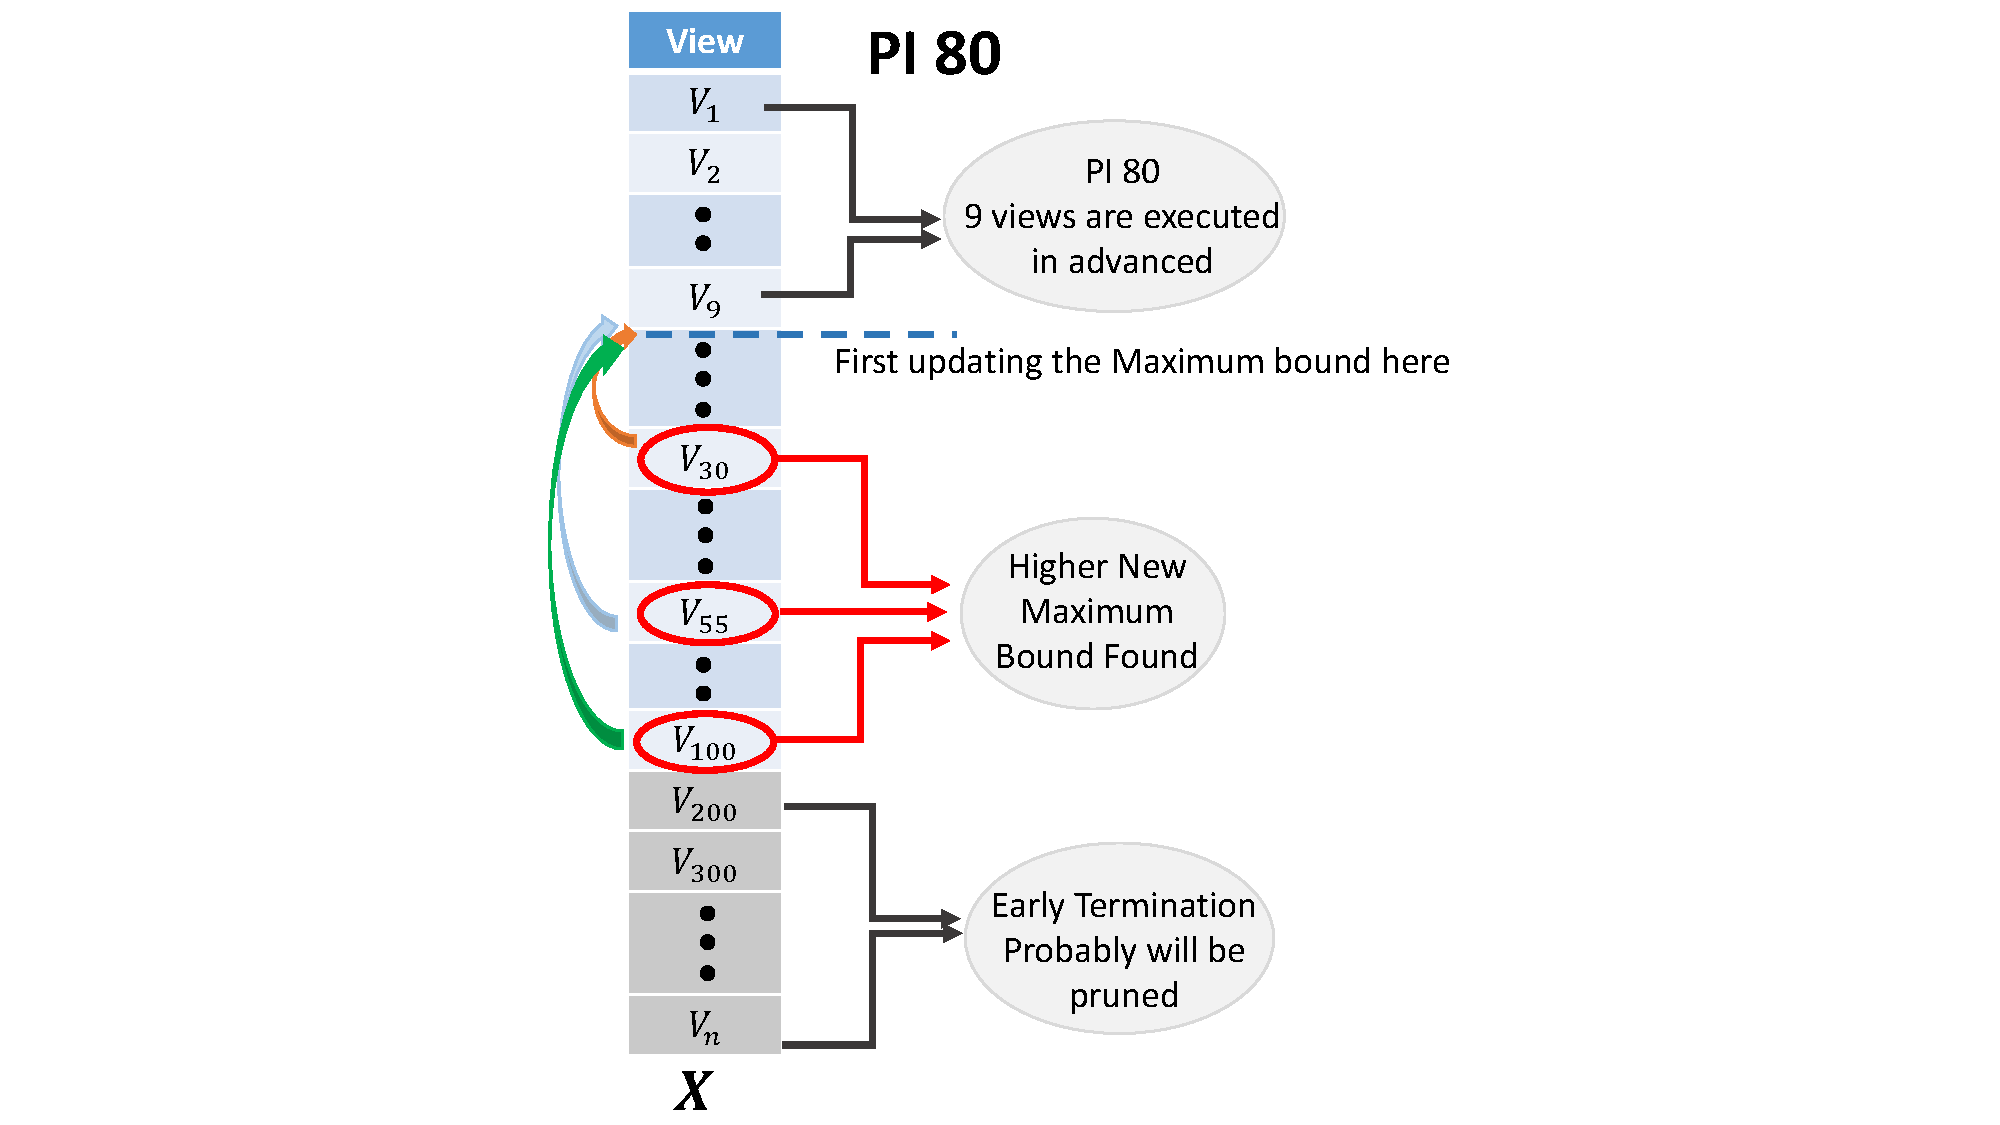
\includegraphics[width=7.0in]{figures/rectifying_bound_2}
%		\vspace{-8pt}
%		\caption{Rectifying maximum bound on adaptive pruning scheme}
%		\label{fig:rectifying_bound_2}
%		
%	\end{center}
%\end{figure}


%As shown in the Figure \ref{fig:DiVE-Greedy} and \ref{fig:adaptive-pruning-performance}, the adaptive bound has a better performance of pruning compared to the static one. 

Our experiment results show that Adaptive scheme has the best pruning performance while PI80 is used. However, it reduces the effectiveness of recommended views due to only small number of executed views are needed for PI80 which increase probability to have wrong bound. The safest way is to use higher PI such as PI95 or PI97. However, if there is a way to keep using PI80 without reducing effectiveness, it will definitely be very good. In fact, \textit{the goal of pruning scheme is to minimize query view execution (i.e., use low PI) without reducing the quality of recommended views}. 


In order to overcome this issue, rectifying bound of adaptive pruning is proposed. The algorithms of our rectifying bound can be seen in algorithm \ref{DiVE-Greedy-Pruning-Rectifying} for DiVE-Greedy-Adaptive and \ref{DiVE-dSwap-Pruning-Rectifying} for DiVE-dSwap-Adaptive.  


The results of this rectifying bound strategy can be seen in Figure \ref{fig:rectifying_bound_greedy_dswap} and Figure \ref{fig:error_fs_adaptive}. Figure \ref{fig:rectifying_bound_greedy_dswap} shows the performance of adaptive pruning scheme with rectifying bound strategy compared to without rectifying bound strategy. The pruning peformance after applying rectifying bound strategy quite close to without rectifying bound strategy. Meanwhile, as shown in Figure \ref{fig:error_fs_adaptive} there is no effectiveness loss after rectifying bound is implemented. 

%
%\begin{figure}
%	\begin{center}
%		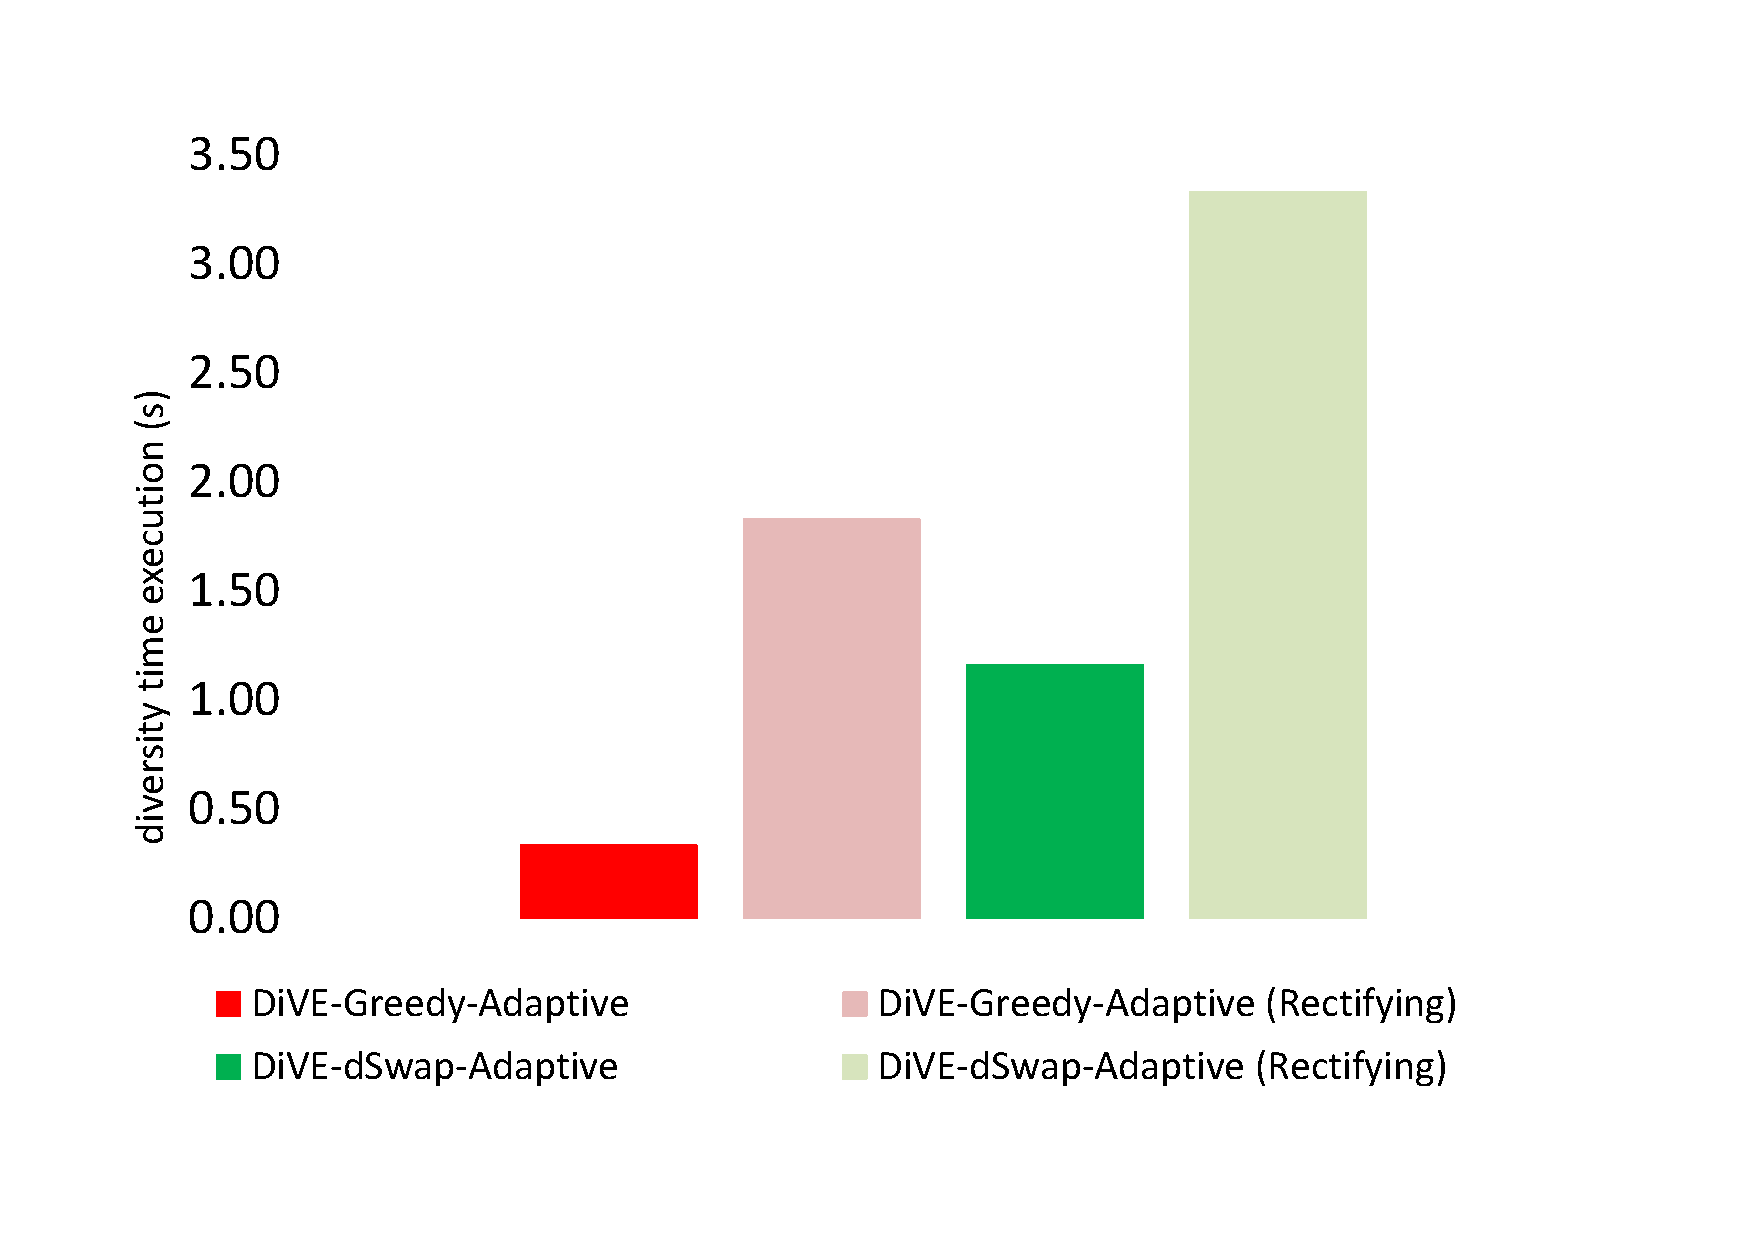
\includegraphics[width=4.0in]{figures/rectifying_cost}
%		\vspace{-8pt}
%		\caption{Rectifying bound strategy cost, $k = 5, \lambda = 0.5$}
%		\label{fig:rectifying_cost}
%		
%	\end{center}
%\end{figure}



%\begin{figure}
%	\begin{center}
%		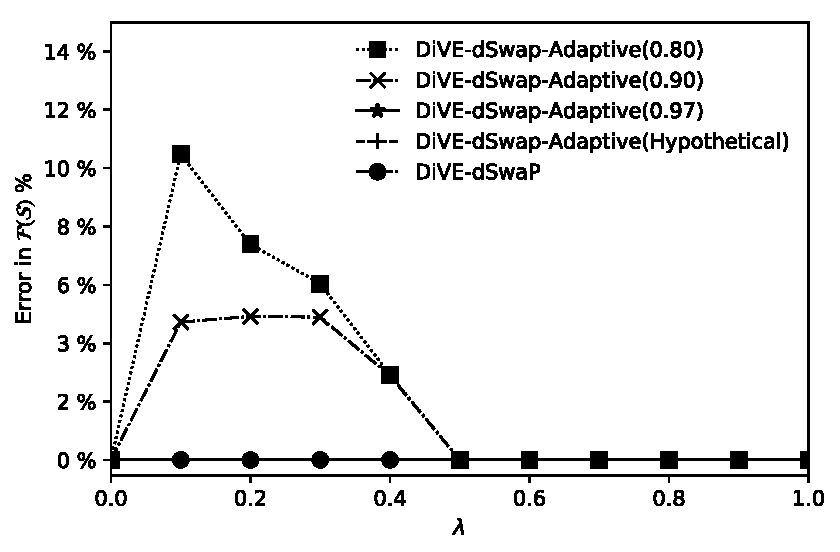
\includegraphics[width=4.0in]{figures/error_f_s}
%		\vspace{-12pt}
%		\caption{Impact of $k$ to diversity computation running on Flights dataset}
%		\label{fig:error_fs_adaptive}
%		
%	\end{center}
%\end{figure}


\section{Total cost with and without Rectifying mechanism}
In the previous report, there is Figure that shows the performance of our proposed pruning approach, especially compared to schemes without pruning. In this report, Figure \ref{fig:flight_costs_all_rectifying} shows the total cost of our pruning scheme with and without rectifying bound strategy running on Flights dataset. 

\begin{figure}
	\begin{center}
		
		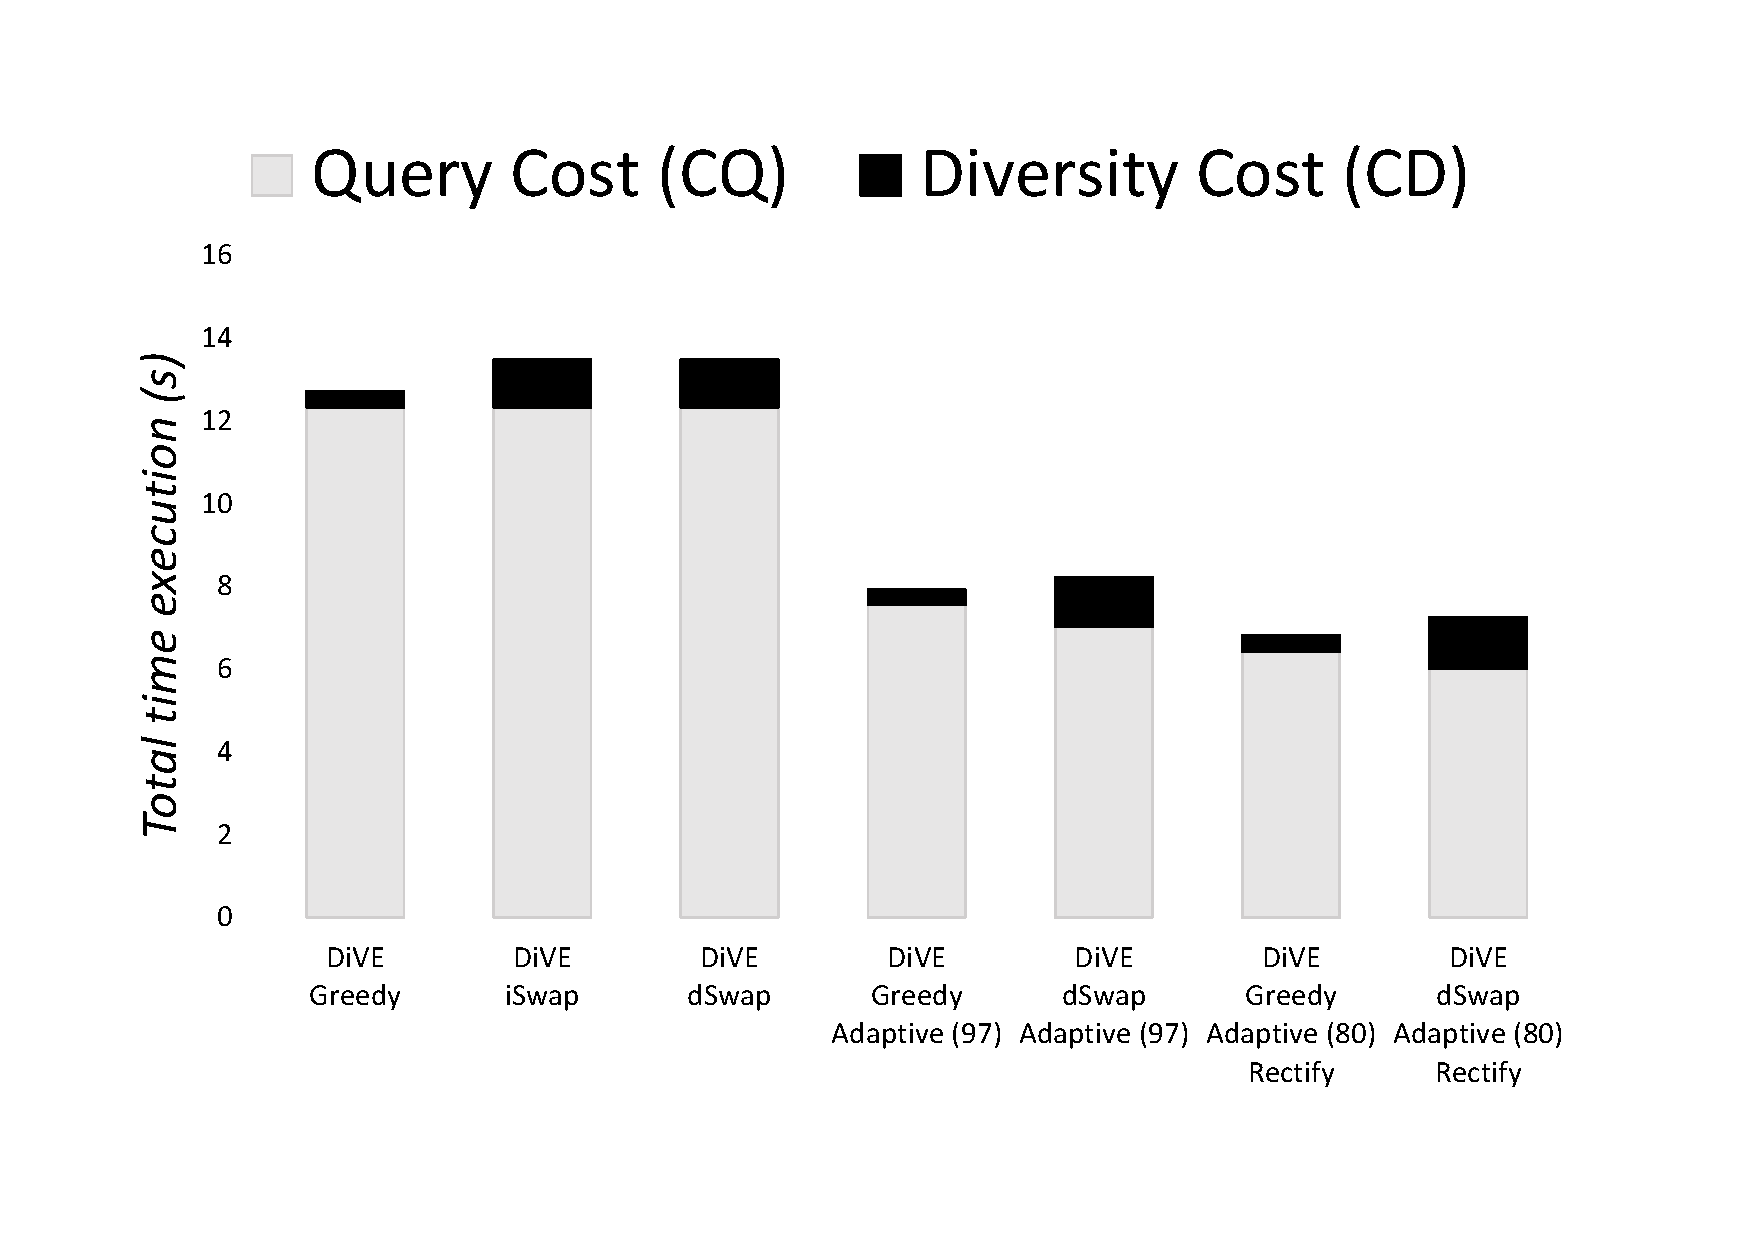
\includegraphics[width=7.0in]{figures/flight_costs_rectifying}
		\vspace{-40pt}
		\caption{Total costs of schemes running on Flights dataset, $k = 5$, and $\lambda = 0.5$ }
		\label{fig:flight_costs_all_rectifying}
		\vspace{-10pt}
	\end{center}
\end{figure}

\begin{figure}
	\begin{center}
		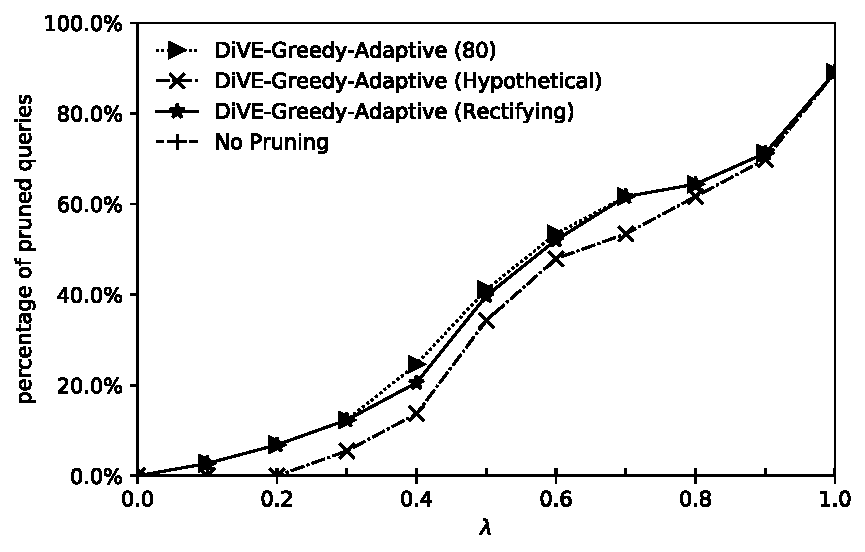
\includegraphics[width=3.0in]{figures/pruning_performance_greedy_rectifying}
		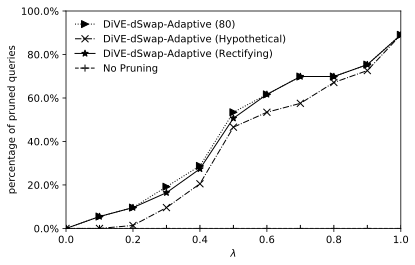
\includegraphics[width=3.0in]{figures/pruning_performance_dswap_rectifying}
		\caption{Pruning performance of rectifying bound schemes compared to others}
		\label{fig:rectifying_bound_greedy_dswap}
	\end{center}
\end{figure}

\begin{figure}
	\begin{center}
		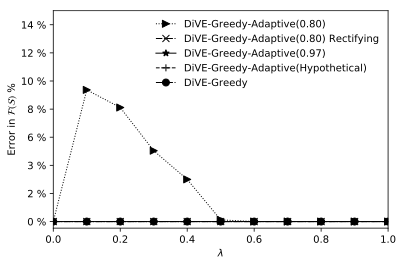
\includegraphics[width=3.0in]{figures/rectifiying_error_f_s_greedy}
		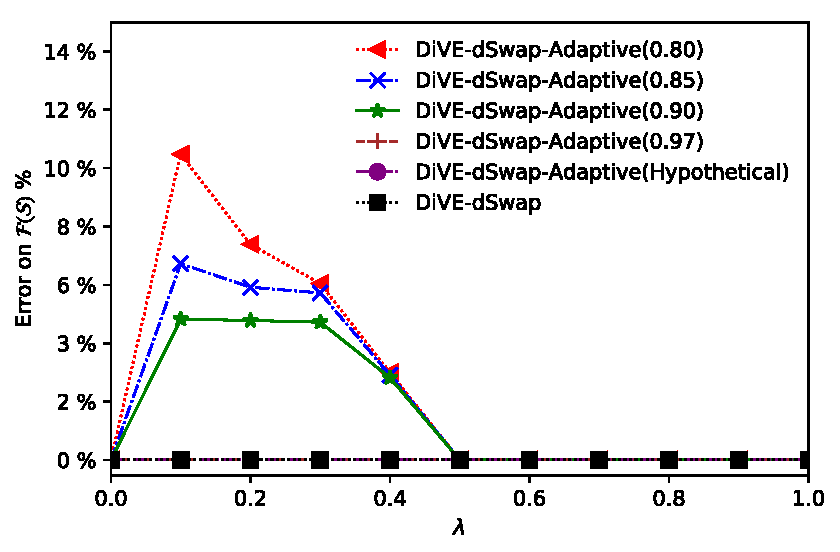
\includegraphics[width=3.0in]{figures/rectifiying_error_f_s_dswap}
		\caption{Error $F(S)$ after rectifying bound}
		\label{fig:error_fs_adaptive}
	\end{center}
\end{figure}



\end{document}



\begin{algorithm}
	\SetAlgoVlined
	\DontPrintSemicolon
	%This is to hide Begin keyword
	\SetKwBlock{Begin}{}{end}
	\KwIn{Set of views V and result set $S$ize k }
	\KwOut{Result set $ S \geq V $, size S = k}  
	\SetKwFunction{FgetL}{getL}
	\SetKwFunction{FgetMaxPI}{getMaxPI}
	$S \leftarrow $ two most distant views\;
	$X \leftarrow  \left[V \backslash S\right]$\;
	
	
	
	\SetKwFunction{FgetL}{getL}
	\SetKwProg{Fn}{function}{:}{}
	\Fn{\FgetL{$f$,$S$, $X$,$L$}}{
		\For{$X_i$ in set $X$}{
			\For{$S_j$ in set $S$}{
				$ d  \leftarrow setDist\left(X_i,S \right) $\;
				$ 	X' \leftarrow [ X_i, d]$\;
				$ 	L.append(X')$\;
			}
		}
		$ 	L \leftarrow sorted\_by\_d(L) $\;
		
		\KwRet\;
	}
	
	\SetKwFunction{FgetMaxPI}{getMaxPI}
	\SetKwProg{Fn}{function}{:}{}
	\Fn{\FgetMaxPI{$f$,$S$, $X$,$max_b$}}{
		$samples \leftarrow get\_samples\_PI(X)$\;
		$maxI\_S \leftarrow get\_maxI(S)$\;
		$maxI\_samples \leftarrow get\_maxI(samples)$\;
		
		\If{ $ maxI\_S > maxI $}{
			$ maxI \leftarrow maxI\_S$
		}
		\If{ $ maxI\_samples> maxI $}{
			$ maxI \leftarrow maxI\_samples$
		}
		$max_b \leftarrow maxI$		
		
		\KwRet\;
	}
	
	$ rectify \leftarrow False $\;
	$ S_{rectify}, L_{rectify}   \leftarrow S, getL(S,X) $\;
	$max_b \leftarrow getMaxPI(S,X) $	\;
	\;
	\While{$i < k$}{
		
		
		
		
		
		
		\For{$L_i$ in $L$}{
			
			\If{ $ F\left(S'\right) < F\left(S \cup X_i, max_b\right) $}{
				$ 	L'.append(L_i)$\;
			}
			$ I \leftarrow get\_I\_score(L'_i) $\;
			\If{ $ F\left(S'\right) < F\left(S \cup X_i, I\right) $}{
				$ S'  \leftarrow S \cup X_i $  \;
			}
			\eIf{ $ I > max_b $}{
				$ max_b \leftarrow I $\;
				$ rectify = True $\;
				$ break (Out\ of\ Loop) $\;
			}{
				$ rectify = False $\;
			}
			
		}
		
		
		
		\eIf{rectify == True}{
			$ S, S' \leftarrow S_{rectify} $ \;
			$ L \leftarrow L_{rectify} $ \;
			$i \leftarrow  len(S)$ \;
			
			
		}{
			
			
			\If{ $ F\left(S'\right) > F\left(S\right) $}{
				$ S  \leftarrow S'$\;
				
			}
			$ S' \leftarrow S $\;
			$ L \leftarrow getL(S,X) $\;
			$i = i + 1  $
			
		}
		
		
		%
		%\If{ $ F\left(S'\right) > F\left(S\right) $}{
		%	$ S  \leftarrow S'$
		%	$  improve \leftarrow  True $\;
		%	
		%	}{
		%		$improve \leftarrow  False $\;
		%	
		%	}
	}
	$return S$
	\caption{\textit{DiVE} Greedy Pruning Rectifying}\label{DiVE-Greedy-Pruning-Rectifying}
\end{algorithm}


% Pruning Pseudocode

\begin{algorithm}
	\SetAlgoVlined
	\DontPrintSemicolon
	%This is to hide Begin keyword
	\SetKwBlock{Begin}{}{end}
	\KwIn{Set of views V and result set $S$ize k }
	\KwOut{Result set $ S \geq V $, size S = k}  
	\SetKwFunction{FgetL}{getL}
	$S \leftarrow $ Result set of only diversity\;
	$X \leftarrow  \left[V \backslash S\right]$\;
	
	
	
	\SetKwFunction{FgetL}{getL}
	\SetKwProg{Fn}{function}{:}{}
	\Fn{\FgetL{$f$,$S$, $X$,$L$}}{
		\For{$X_i$ in set $X$}{
			\For{$S_j$ in set $S$}{
				$ d  \leftarrow setDist\left(X_i,S \backslash S_j\right) $\;
				$ 	X' \leftarrow [S_j, X_i, d]$\;
				$ 	L.append(X')$\;
			}
		}
		$ 	L \leftarrow sorted\_by\_d(L) $\;
		
		\KwRet\;
	}
	
	\SetKwFunction{FgetMaxPI}{getMaxPI}
	\SetKwProg{Fn}{function}{:}{}
	\Fn{\FgetMaxPI{$f$,$S$, $X$,$max_b$}}{
		$samples \leftarrow get\_samples\_PI(X)$\;
		$maxI\_S \leftarrow get\_maxI(S)$\;
		$maxI\_samples \leftarrow get\_maxI(samples)$\;
		
		\If{ $ maxI\_S > maxI $}{
			$ maxI \leftarrow maxI\_S$
		}
		\If{ $ maxI\_samples> maxI $}{
			$ maxI \leftarrow maxI\_samples$
		}
		$max_b \leftarrow maxI$		
		
		\KwRet\;
	}
	
	
	$ F_{current}, improve, rectify \leftarrow  0, True, False $\;
	$ S_{rectify}, L_{rectify}   \leftarrow S, getL(S,X) $\;
	$max_b \leftarrow getMaxPI(S,X) $	\;
	\;
	\While{improve = True}{
		
		
		\For{$L_i$ in $L$}{
			
			\If{ $ F\left(S'\right) < F\left(S \backslash S_j \cup X_i, max_b\right) $}{
				$ 	L'.append(L_i)$\;
			}
			$ I \leftarrow get\_I\_score(L'_i) $\;
			\If{ $ F\left(S'\right) < F\left(S\backslash S_j \cup X_i, I\right) $}{
				$ S'  \leftarrow S \backslash j \cup X_i $  \;
			}
			\eIf{ $ I > max_b $}{
				$ max_b \leftarrow I $\;
				$ rectify = True $\;
				$ break (Out\ of\ Loop) $\;
			}{
				$ rectify = False $\;
			}
			
		}
		
		
		
		\eIf{rectify == True}{
			$ S, S' \leftarrow S_{rectify} $ \;
			$ L \leftarrow L_{rectify} $ \;
			$improve \leftarrow  True$ \;
			
			
		}{
			
			
			\If{ $ F\left(S'\right) > F\left(S\right) $}{
				$ S  \leftarrow S'$\;
				
			}
			
			\eIf{ $ F\left(S\right) > F_{current} $}{
				$ F_{current}  \leftarrow F\left(S\right) $\;
				$  improve \leftarrow  True $\;
				
			}{
				$improve \leftarrow  False $\;
				
			}
			$ S' \leftarrow S $\;
			$ L \leftarrow getL(S,X) $\;
			
		}
		
		%
		%\If{ $ F\left(S'\right) > F\left(S\right) $}{
		%	$ S  \leftarrow S'$
		%	$  improve \leftarrow  True $\;
		%	
		%	}{
		%		$improve \leftarrow  False $\;
		%	
		%	}
	}
	$return S$
	\caption{\textit{DiVE} dSwap Pruning Rectifying}\label{DiVE-dSwap-Pruning-Rectifying}
\end{algorithm}


% Pruning Pseudocode

\begin{algorithm}
	\SetAlgoVlined
	%This is to hide Begin keyword
	\SetKwBlock{Begin}{}{end}
	\KwIn{Set of views V and result set $S$ize k }
	\KwOut{Result set $ S \geq V $, size S = k}  
	$S \leftarrow $ Result set of only diversity\;
	$X \leftarrow  \left[V \backslash S\right]$\;
	$F_{current} \leftarrow 0 $\;
	$  improve \leftarrow  True $\;
	$ max_b  \leftarrow\sqrt{2} $\;
	%$ S_{rectify}  \leftarrow [] $\;
	%$ X_{rectify}  \leftarrow [] $\;
	\While{improve = True}{
		%$ X' \leftarrow [] $\;
		\For{$X_i$ in set $X$}{
			\For{$S_j$ in set $S$}{
				$ d  \leftarrow setDist\left(X_i,S \backslash S_j\right) $\;
				$ 	newX \leftarrow [S_j, X_i, d]$\;
				$ 	X'.append(newX)$\;
			}
		}
		$ 	X' \leftarrow sorted\_by\_d(X') $\;
		$ S' \leftarrow S $\;
		$ rectify  = False $\;
		\eIf{ $ max_b == \sqrt{2} $}{
			\For{$i$ in set $X'$}{
				
				\If{ $ F\left(S'\right) < F\left(S \backslash X'[i][0] \cup X'[i][1], max_b\right) $}{
					$ 	X''.append(X'[i][1])$\;
				}
			}
			
			$n \leftarrow pi - len(S)$\;
			$samples \leftarrow X''[0\colon n]$\;
			$maxI\_S \leftarrow get\_maxI(S)$\;
			$maxI\_samples \leftarrow get\_maxI(samples)$\;
			
			\If{ $ maxI\_S > maxI $}{
				$ maxI \leftarrow maxI\_S$
			}
			\If{ $ maxI\_samples> maxI $}{
				$ maxI \leftarrow maxI\_samples$
			}
			$max\_b \leftarrow maxI$	
			
			\For{$i$ in set $X''$}{
				\For{$j$ in set $S$}{
					\If{ $ F\left(S'\right) < F\left(S \backslash S_j \cup X''[i], max_b\right)  $}{
						$ 	X'''.append(X''[i])$\;
						
					}
					$ I \leftarrow get\_I\_score(X'''[i]) $\;
					\If{ $ F\left(S'\right) < F\left(S \backslash S_j \cup X'''[i], I\right) $}{
						$ S'  \leftarrow S \backslash j \cup X'''[i] $  \;
					}
					\If{ $ I > max_b $}{
						$ max_b \leftarrow I $\;
						$ rectify = True $\;
						$ break (Out\ of\ Loop) $\;
					}
				}
			}
			
		}{ 
			
			
		}
		%
		%\If{ $ F\left(S'\right) > F\left(S\right) $}{
		%	$ S  \leftarrow S'$
		%	$  improve \leftarrow  True $\;
		%	
		%	}{
		%		$improve \leftarrow  False $\;
		%	
		%	}
	}
	%return S
	\caption{\textit{DiVE} dSwap Pruning Rectifying}\label{DiVE-dSwap-Pruning-Rectifying}
\end{algorithm}

\begin{algorithm}
	\LinesNumbered
	\setcounter{AlgoLine}{37}
	% This is to restore vline mode if you did not take the package as \usepackage[linesnumbered,ruled,vlined]{algorithm2e}
	\SetAlgoVlined
	%This is to hide Begin keyword
	\SetKwBlock{Begin}{}{end}
	\Begin{
		\eIf{...}{...}
		{
			
			\For{$X_i$ in set $X'$}{
				\If{ $ F\left(S'\right) < F\left(S \backslash X'[i][0] \cup X'[i][1], max_b\right) $}{
					$ 	X''.append(X'[i][1])$\;
				}
				$ I \leftarrow get\_I\_(X''[i]) $\;
				\If{ $ F\left(S'\right) < F\left(S \backslash S_j \cup X''[i], I\right) $}{
					$ S'  \leftarrow S \backslash j \cup X''[i] $  \;
				}
				\If{ $ I > max\_b $}{
					$ max\_b \leftarrow I $ \;
					$ rectify = True $\;
					$ break (Out\ of\ Loop) $\;
				}
				
			}
			
		}
		
		\eIf{rectify == True}{
			$improve \leftarrow  True$ \;
			
			
		}{
			
			
			\If{ $ F\left(S'\right) > F\left(S\right) $}{
				$ S  \leftarrow S'$\;
				
			}
			
			\eIf{ $ F\left(S\right) > F_{current} $}{
				$ F_{current}  \leftarrow F\left(S\right) $\;
				$  improve \leftarrow  True $\;
				
			}{
				$improve \leftarrow  False $\;
				
			}
			
		}
		
	}   
	$return S$ 
\end{algorithm}


\SetKwFunction{FgetNewS}{getNewS}
\SetKwProg{Fn}{function}{:}{}
\Fn{\FgetNewS{$f$,$S$, $X$,$max_b$, $G$}}{
	$ S' \leftarrow S $\;
	\For{$L_i$ in $L$}{
		
		\If{ $ F\left(S'\right) < F\left(S \cup X_i, max_b\right) $}{
			$ I \leftarrow get\_I\_score(X_i) $\;
			\If{ $ F\left(S'\right) < F\left(S \cup X_i, I\right) $}{
				$ S'  \leftarrow S \cup X_i $  \;
			}
			\eIf{ $ I > max_b $}{
				$ max_b \leftarrow I $\;
				$ rectify = True $\;
				$ break (Out\ of\ Loop) $\;
			}{
				$ rectify = False $\;
				
			}
			
			
		}
		
		
	}
	\If{ $ F\left(S'\right) > F\left(S\right) $}{
		$ S  \leftarrow S'$\;
	}
	$ G  \leftarrow S, rectify $\;
	\KwRet G\;
}


%\section{Proposed algorithm's Figure}
%We proposed DiVE scheme using two kinds of popular heuristic approach which are Greedy and Swap techniques. Figure \ref{fig:algorithm-figure} shows our proposed scheme technique. In case of Greedy, the set $ S $ is initialized by two most distant views. In each iteration, the best view in $ X $ that can maximize objective function $F(S)$ will be added to the set $ S $. Meanwhile, for the Swap case, the set $ S $ is initialized by the most diverse $  k $ views and in each iteration, all candidates views in $ X $ will be interchanged to set $ S $ and view which can improve the current objective function $F(S)$ will replace a view in set $ S $.
%
%The $setDist$ score is used to sort all candidate views in $ X $, the highest score means that views is more diverse to set $ S $. The current bound is utilized to compute the estimate utility of each candidate view. First, the theoritical maximum bound ($ \sqrt{2} $) is used and this bound is updated while the actual importace score of view has been known. To avoid the wrong current bound, samping based on prediction interval is used. Before running the program, user needs to defined what PI that she wants to use. For instance, while users set PI to 80 then after 9 views is executed the current bound will be updated to the maximum bound which have seen so far. The most used PI can be defined as following: 
%
%\begin{itemize}[noitemsep]
%	\item PI80: need to execute 9 views
%	\item PI85: need to execute 12 views
%	\item PI90: need to executes 20 views
%	\item PI95: need to executes 40 views
%	\item PI97: need to executes 60 views
%\end{itemize}
%
%
%\begin{figure}
%	\begin{center}
%		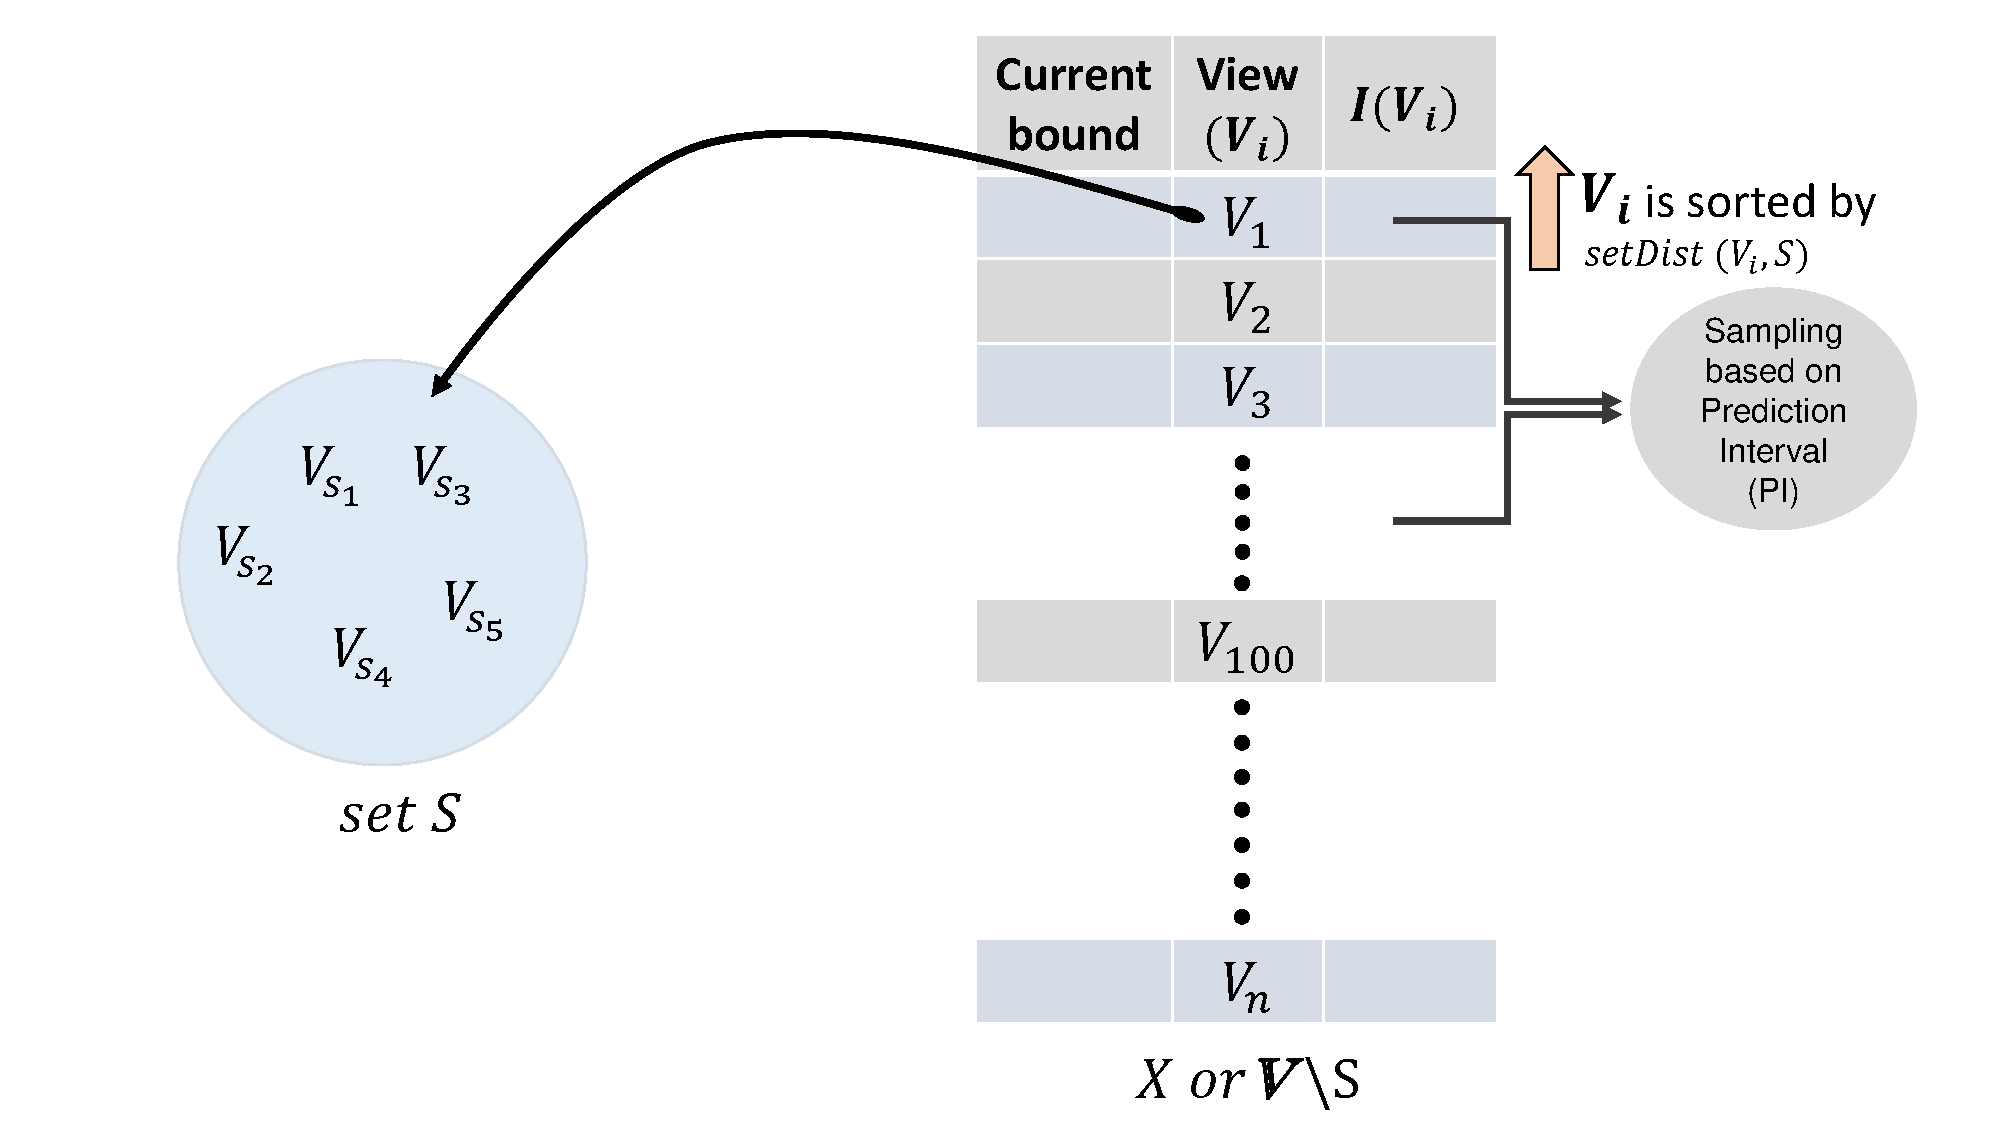
\includegraphics[width=5.0in]{figures/Algorithm}
%		\vspace{-12pt}
%		\caption{Utilizing $setDist$ score to sort candidate views and update current maximum bound to optimize the pruning performance}
%		\label{fig:algorithm-figure}
%		
%	\end{center}
%\end{figure}


%For the general case, Euclidean distance $d$ is defined as following: 
%$d = \sum{(x-y)^2} = \sum x^2 + \sum y^2 - 2\sum xy$. Given that in probability vectors all values are nonnegative, $d$ is max when the last term is zero, then $d = \sum x^2 + \sum y^2$.
%
%All values are between 0 and 1 (sum up to 1), $\sum x = \sum y = 1$. In such a vector, its theoretical maximum is attained when all its entries are 0 except one which is 1, it is when $\sum x^2 = \sum x$ and $\sum y^2 = \sum y$. It also follows from the above description, that then $\sum xy$ can very easily happen to be zero (since in each vector there is just single nonzero element).
%\newline

%Example maximum condition for two bins case: 
%\newline
%
%$\sum a = \sum b = 1$, $a , b \geq 0$
%\newline
%
%$(\sum a)^2 + (\sum b)^2 \geq \sum a^2 + \sum b^2$
%\newline
%
%$(\sum a)^2 + (\sum b)^2 \geq \sum a^2 + \sum b^2 - \sum 2ab $ 
%\newline
%
%$(\sum a)^2 + (\sum b)^2 \geq \sum (a^2 +  b^2 -  2ab)  $ 
%\newline
%
%$(\sum a)^2 + (\sum b)^2 \geq \sum (a-b)^2  $ 
%\newline
%
%$1 + 1 \geq \sum (a-b)^2  $ 
%\newline
%
%$\sqrt{2} \geq \sqrt{\sum (a-b)^2}  $ 
%\newline

%Max-sum is bi-criteria objective function to maximize the sum of the relevance and dissimilarity of the selected set, which can be defined as follows:
%
%\begin{equation}
%F\left(S\right) =  \left(1-\lambda\right) * I\left(S\right) + \lambda * f\left(S,D\right)
%\label{objectif_function}
%\end{equation}
%
%Where, 
%$ I\left(S\right)= \sum_{i=1}^{k} \dfrac{I(V_i )}{I_u}, V_i  \in S $ and $ f\left(S,D\right)= \dfrac{1}{k\left(k-1\right)}  \sum_{i=1}^{k} \sum_{j>i}^{k} D\left(V_i,V_j\right) ,V_i,V_j  \in S $
%\newline
%
%Meanwhile, Max-min diversification is the bi-criteria objective function that maximize the \textit{minimum} relevance and dissimilarity of the selected set. Based on the work of Gollapudi (An axiometic approach for result diversificaiton), this objective function can be defined as follows: 
%
%\begin{equation}
%F\left(S\right) = (1-\lambda) * \underset{u \in S} {\mathrm{min}} \ w\left(u\right)  + \lambda * \underset{u,v \in S} {\mathrm{min}} d\left(u,v\right)
%\end{equation}
%
%While Max-min diversification is to maximize the minimum of importance score, I am not sure this approach is relevant or not for our work. 